\documentclass{article}

\usepackage{neurips_2026}

\usepackage[utf8]{inputenc}
\usepackage[T1]{fontenc}
\usepackage{hyperref}
\usepackage{url}
\usepackage{booktabs}
\usepackage{amsfonts}
\usepackage{amsmath}
\usepackage{amssymb}
\usepackage{nicefrac}
\usepackage{microtype}
\usepackage{xcolor}
\usepackage{graphicx}
\usepackage{subcaption}
\usepackage{multirow}
\usepackage{enumitem}
\usepackage{pgfplots}
\pgfplotsset{compat=1.18}
\usepackage{algorithm}
\usepackage{algpseudocode}

\newcommand{\todo}[1]{\textcolor{red}{\textbf{[TODO: #1]}}}
\newcommand{\am}[1]{\textcolor{blue}{{[aneesh: #1]}}}
\newcommand{\dc}[1]{\textcolor{teal}{{[dylan: #1]}}}
\newcommand{\Kset}{\{1,2,3,4\}}
\newcommand{\pigate}{\pi_{\mathrm{gate}}}


\title{Planning in Real-Time Reinforcement Learning}

Reinforcement learning for budgeting MCTS planning under real-time

Reinforcement learning for budgeting computation in real-time

\author{\todo{Author list}}


\begin{document}

\maketitle

% =============================================================================
\begin{abstract}
% =============================================================================

Deliberating takes time, and in real-time settings that time is not free.
Standard reinforcement learning (RL) sidesteps this, as the environment waits indefinitely
for the agent's decision, so computation is costless.
We study environments where this assumption fails, where the environment progresses
while the agent plans, and the cost of deliberation is paid in outcomes rather than
wall-clock seconds.
We train a lightweight meta-policy that decides how much computation to invest at each step.
The meta-policy consistently outperforms every fixed-budget baseline while using
less average compute.
Moreover, we validate the full pipeline in a true two-GPU real-time setup. We demonstrate these results across real-time Pac-Man, Tetris, Snake, timed Sokoban,
and two-player speed Hex.

\end{abstract}


% =============================================================================
\section{Introduction}
% =============================================================================

Expert decision-makers do not think equally hard about every choice.
A chess player under time pressure blitzes most moves and reserves deliberation for
critical board positions.
A skilled Tetris player barely pauses on easy placements but slows when the board
grows dense.
This adaptive allocation of cognitive effort is so natural, yet it is entirely absent from the standard reinforcement learning (RL) framework \cite{travnik2018reactive, ramstedt2019rtrl}.

In standard RL the environment waits. The agent may deliberate indefinitely before
committing to an action, and computation time carries no cost whatsoever.
Real-time settings break this assumption. The world keeps progressing while the agent plans.
The cost of deliberation is not wall-clock latency but steps taken by
the environment while the agent is still deciding. A perfect action computed
one moment too late may be far worse than a timely, good-enough action.

This creates a spectrum of decision-making regimes.
At one extreme, every frame demands an immediate reaction with no time to deliberate.
At the other, the environment is fully paused and thinking is costless (the setting
standard RL was designed for).
Between these poles lies a rich, underexplored regime of environments where more
planning reliably improves decisions, but at an environment cost that grows with the depth of that
planning.

We study this intermediate regime using planning-based agents. Specifically,
AlphaZero-style models~\cite{silver2018general} that use Monte Carlo Tree Search (MCTS)
to improve action selection with additional computation
(see Appendix~\ref{app:az_primer} for a self-contained primer).
In MCTS, an agent repeatedly simulates plausible continuations from the current state,
guided by a neural network that predicts action probabilities and state values;
each additional simulation refines the estimate of which action is best.
A key property is that more simulations reliably improve decision quality,
at the direct cost of more compute and, in real-time settings, more elapsed game time.
As an agent plans more, it performs better. But planning also takes time, and in
real-time settings that time is paid directly in game outcomes. This dual property
(planning quality scales up with compute, and real-time cost scales up with inference
time) makes adaptive compute allocation the natural lever for performance.

We train a lightweight \emph{gating policy} that reads the current game state and
the planner's own value estimate and intermediate features to choose a planning depth
at each decision point.
While the planner runs in the background, the agent takes \emph{committed actions}.
In committed-action environments these are fast reflex actions sampled from the logits of our reflex policy
that keep the agent moving without full deliberation; in
clock environments, where the board does not evolve while a player thinks, they
are no-ops that simply consume the player's clock.
The gating policy learns to allocate computation to the moments where it matters most
and to act quickly everywhere else.

Our contributions are:
\begin{enumerate}
  \item \textbf{Real-time RL environment design.}
    We identify two complementary design patterns for real-time environments:
    \emph{committed-action progression} (the agent takes reflex actions while
    a slower planner computes) and \emph{explicit clocks} (a per-player timer
    depleted by thinking time).
    In both cases, the planning process is cost-aware by construction.
  \item \textbf{Planning quality vs.\ inference time.}
    We empirically characterize how planning quality and real-time inference cost
    co-scale with simulation count, establishing the joint tradeoff that motivates
    adaptive allocation.
  \item \textbf{Adaptive gating policy.}
    We formulate planning-depth selection as a variable-duration meta-decision problem
    and train a lightweight gating network on top of a frozen planner.
    The gating policy selects a depth $K \in \Kset$, determining the simulation budget
    and, in committed-action environments, the number of fast reflex actions taken
    while the planner runs.
\end{enumerate}

We substantiate these contributions empirically. Across all five environments,
the gating policy outperforms every fixed-depth baseline while using less
average compute, and the learned strategy concentrates deliberation in
high-stakes situations in interpretable, state-dependent ways. We further
validate the approach in a true two-GPU real-time setup, with the environment running on one GPU and MCTS on a second. Because
training already simulates the planning delay by executing $K{-}1$ committed
actions while MCTS searches in parallel, the trained gating policy transfers
directly to asynchronous deployment with no retraining and no architectural
changes.

% =============================================================================
\section{Background and Related Work}
% =============================================================================

\paragraph{Deliberation has always had a cost.}
The idea that thinking takes time, and that this time has value, predates deep
RL by decades. Russell and Wefald's value-of-computation~\cite{russell1991right}
formalised when an additional computation is worth its cost; the anytime
planning literature~\cite{korf1990rta,dean1988analysis,zilberstein1996using,likhachev2003ara}
built algorithms around the resulting tradeoff. Applied to MCTS, this
perspective casts simulation selection as a meta-level decision
problem~\cite{hay2012selecting,tolpin2012simple,sezener2020static,lin2015metareasoning},
and the cogsci revival~\cite{lieder2017strategy,griffiths2019doing,callaway2018learning}
casts bounded-optimal cognition itself as a metalevel MDP. The question this
literature poses, how much should the agent deliberate, given that
deliberation is costly?, is the question we ask in deep RL.

\paragraph{Modern deep RL has mostly sidestepped it.}
AlphaZero-family planners~\cite{silver2018general,schrittwieser2020muzero}
treat MCTS budget as a fixed hyperparameter at deployment, with Gumbel
MuZero~\cite{danihelka2022policy} the notable advance toward small budgets.
Real-time RL~\cite{ramstedt2019rtrl,travnik2018reactive} reintroduces the
cost of deliberation by formalising environments that progress during action
selection, with extensions for action and observation
delays~\cite{walsh2009delayed,derman2021delayed,bouteiller2021random,katsikopoulos2003markov}
and concurrent control~\cite{xiao2020thinking}. Recent work mitigates inference
cost through asynchronous and pipelined
architectures~\cite{riemer2025staggered,anokhin2025handling}. However, across all
of this work, inference cost is something the architecture imposes, not
something the agent reasons about.

\paragraph{Adapting compute per state.}
The closest neighbours to our work \emph{learn} to allocate planning compute. Metacontrol~\cite{hamrick2017metacontrol}
trains a meta-controller to choose how many imagination steps to run; Thinker
and Dynamic Thinker~\cite{chung2023thinker,wang2024dynamic} let the agent
itself decide when to imagine alternative trajectories on top of a learned
world model; Adaptive Lookahead~\cite{dalal2022adaptive} learns a
state-dependent tree-search horizon. ~\cite{hamrick2021role}'s ablation
study provides the strongest empirical motivation: shallow MuZero trees often suffice, and the marginal value of additional
simulations varies sharply by state. In parallel, the LLM community has
independently advanced the same idea: PonderNet and adaptive computation
time~\cite{graves2016act,banino2021pondernet,schuster2022calm} learn per-input
halting; test-time compute scaling~\cite{snell2024scaling,deepseek2025r1,muennighoff2025s1}
and RL-trained reasoning-length
controllers~\cite{aggarwal2025l1,muppidi2025predictive,fang2025thinkless,shen2025dast}
explicitly learn per-query thinking budgets; cascaded
routing~\cite{kim2023bigl,chen2023frugalgpt,ong2025routellm} defers easy
queries to cheap models. The shared thesis is that a small learned policy can
profitably decide how much computation to spend per decision.

\paragraph{Our setting.}
We share this thesis but address a setting none of these works does. We gate
a \emph{frozen} AlphaZero-style planner, requiring no joint training between
meta-policy and planner. The cost of deliberation is paid in
\emph{environmental progress} (ghosts close in, pieces fall, clocks
deplete) not in artificial reward shaping, so the gating policy learns a value-of-computation function from outcomes alone. Moreover, the
committed-action protocol that makes this real-time cost legible during
training also describes the dynamics of true asynchronous execution, so the
trained policy transfers directly to a two-GPU deployment with no
architectural change. Other axes of ``learning to
search''~\cite{guez2018mctsnets,farquhar2018treeqn,hamrick2020save,racaniere2017i2a}
modify the planner's internal behaviour rather than its budget, and the
options framework~\cite{sutton1999between,bradtke1994reinforcement,bacon2017optioncritic,harb2018deliberation}
together with classical MCTS time-management~\cite{baier2016time,huang2010timemanagement,baudis2012pachi}
provide the formal scaffolding for variable-duration meta-decisions and the
baselines for our clock environments.


\section{Real-Time RL Environments}
\label{sec:envs}
% =============================================================================

In a real-time environment the clock runs independently of the agent's decision-making.
Every game tick, the world advances, the Tetris piece falls one row, the Pac-Man
ghosts step, the Hex clock depletes, regardless of whether the agent has finished
deliberating.
Computation time is therefore a direct cost in game outcomes. A more deliberate agent
pays in world-progression steps rather than wall-clock seconds.

Figure~\ref{fig:tetris_committed} illustrates the mechanism for real-time Tetris.
An I-shaped piece spawns at the top of the board.
The gating policy selects $K{=}4$, reserving four game ticks for the planner.
During ticks $t{+}1$ through $t{+}3$, a fast reflex policy ($\pi_{reflex}$)
takes committed actions, here, moving the piece left each tick as gravity pulls it
down.
MCTS runs 128 simulations in the background over those same ticks, simulating the
committed-action trajectory to find the best action for tick $t{+}4$.
It identifies a four-cell gap on the right side of the board and places the piece there
on the final step, a placement the reflex policy would have missed.

\begin{figure}[t]
  \centering
  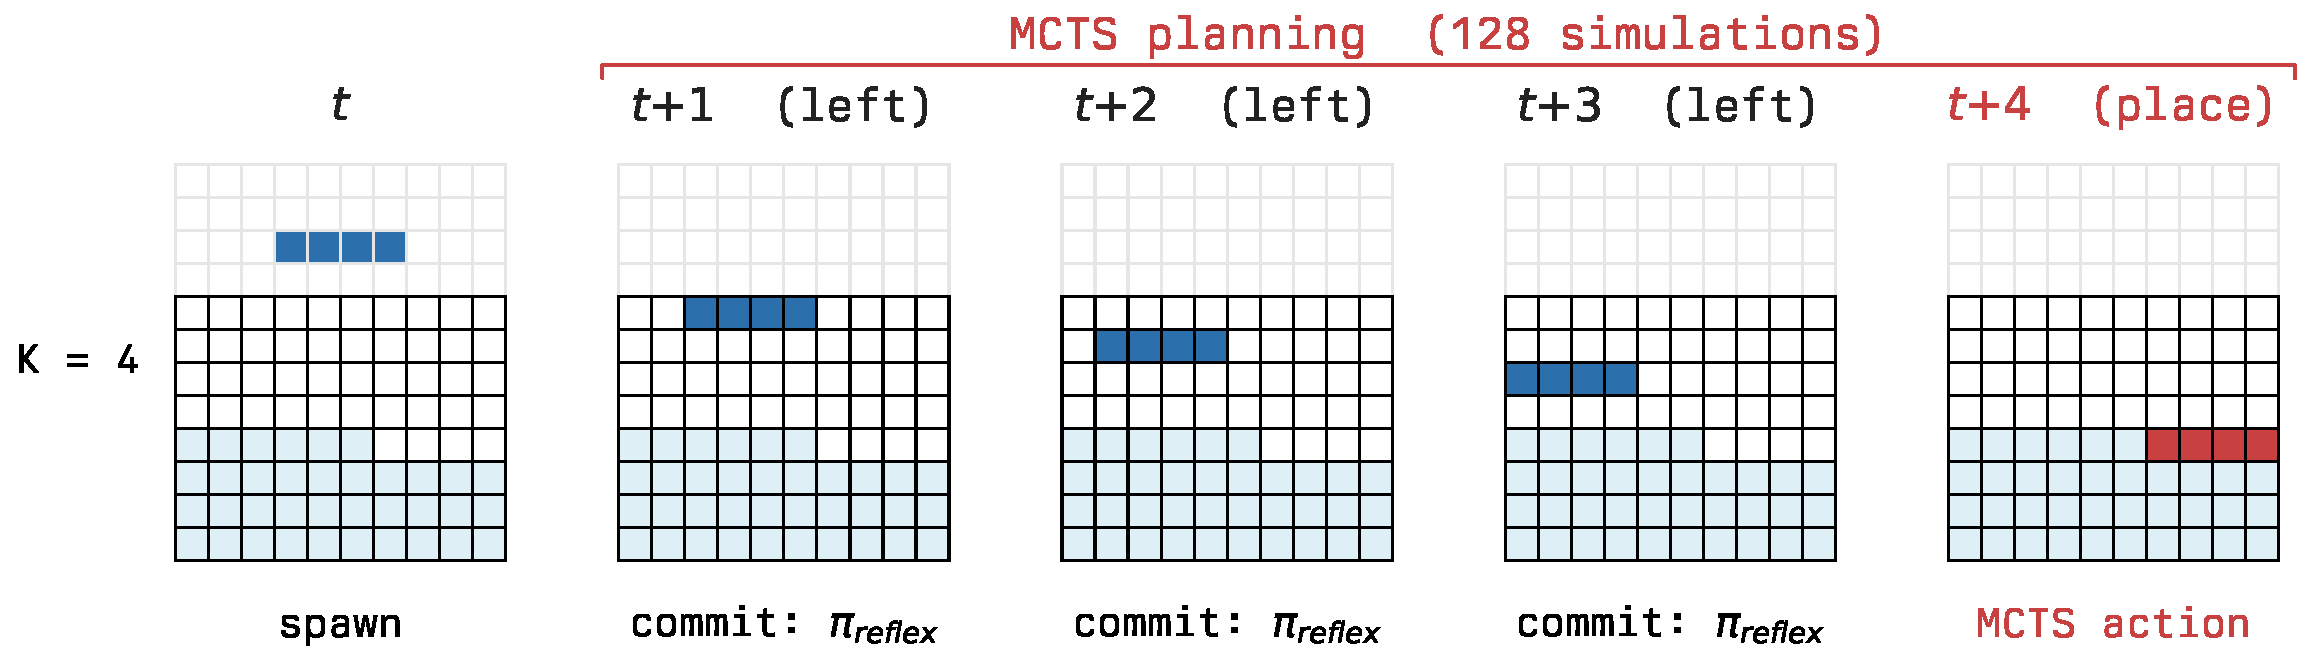
\includegraphics[width=\linewidth]{figures/tetris_committed.pdf}
  \caption{Committed-action execution in real-time Tetris with $K{=}4$.
    The I-piece spawns at top center (light blue).
    Ticks $t{+}1$–$t{+}3$ are committed actions from the reflex policy
    $\pi_{reflex}$ that move the piece left while gravity falls it one row per tick.
    Tick $t{+}4$ (red): the MCTS result fires, having searched 128 simulations
    over the committed-action trajectory, it identifies a four-cell gap on the right
    and places the piece there.
    Piece positions are schematic; the key point is that MCTS plans
    \emph{over} the committed-action delay, not despite it.}
  \label{fig:tetris_committed}
\end{figure}

\begin{figure}[t]
  \centering
  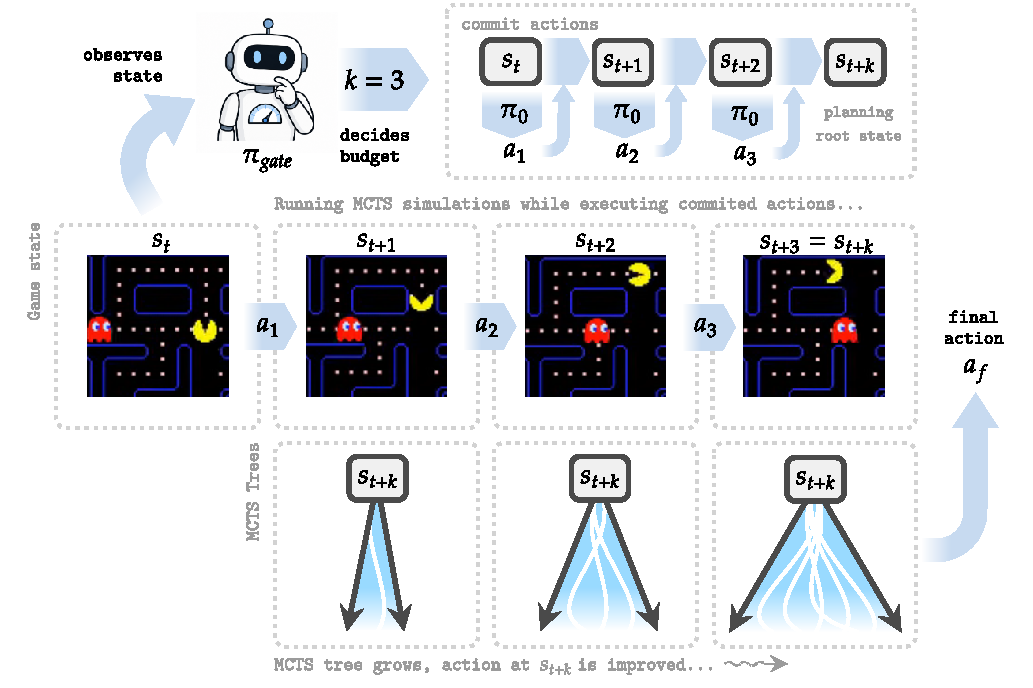
\includegraphics[width=\linewidth]{figures/realtime-rl-gating-diagram.pdf}
  \caption{
    Overview of the gating policy making a decision.
  }
  \label{fig:realtime-rl-gating-diagram}
\end{figure}

Across all the environments we study, the planning process is \emph{cost-aware} by
construction. Either the MCTS tree explicitly simulates how the world evolves during
the planning delay, or the network is trained on observations that include the
remaining time budget, making its value estimates inherently sensitive to the cost of
thinking.
We study two mechanisms through which this property arises.

\subsection{Committed-action environments: Pac-Man and real-time Tetris}

In committed-action environments, acting and planning happen concurrently.
When the gating policy selects a planning depth $K$, it reserves $K$ environment steps
for the planner. The agent takes $K{-}1$ \emph{committed actions}, which are fast reflex actions
decisions drawn from the planner's own policy, while the full planner runs in the
background. On the $K$-th step, the planner's result is applied.
The MCTS tree accounts for this explicitly: its recurrent function simulates the $K{-}1$
committed-action steps, so search is conducted over the same future the agent will
actually experience. The cost of deeper planning is exactly $K{-}1$ additional steps
of world progression before the carefully chosen action lands.

\textbf{Pac-Man~\cite{jumanji2022}.}
Ghosts advance every step regardless of the agent's action.
Committed actions keep the agent moving under a reflex policy while MCTS
computes. A deeper plan means the agent has navigated farther before the MCTS action
fires.

\textbf{Real-time Tetris~\cite{jumanji2022}.}
Gravity advances the falling piece one row every step.
The same committed-action mechanism applies: the agent moves under a reflex policy
policy for $K{-}1$ steps while the planner searches, then the planner's chosen
placement is executed on step $K$.
The piece has descended further when the decision lands, making placement precision
more consequential for deeper plans.

\paragraph{Equal compute budget.}
All depth options $K \in \Kset$ are designed to carry the same per-frame simulation
budget: at depth $K$, the planner runs $K \times 32$ simulations over $K$ environment
steps, so each game frame receives exactly 32 simulations on average (Table~\ref{tab:budget}).
Differences in performance therefore reflect \emph{when} compute is used, not how
much total compute is consumed.


\begin{table}[h]
  \centering
  \caption{Committed-action environments: all $K$ options share 32 MCTS simulations
    per game frame.}
  \label{tab:budget}
  \small
  \begin{tabular}{lcccc}
    \toprule
    & $K{=}1$ & $K{=}2$ & $K{=}3$ & $K{=}4$ \\
    \midrule
    MCTS simulations       & 32 & 64 & 96 & 128 \\
    Committed actions      & 0  & 1  & 2  & 3   \\
    Simulations per frame  & 32 & 32 & 32 & 32  \\
    \bottomrule
  \end{tabular}
\end{table}

\subsection{Clock environments: speed Hex and timed Sokoban}

In clock environments, the agent's remaining time is part of the observation and the
network is trained to be budget-aware.
MCTS simulations operate on board-only dynamics (no clock deduction during search),
but because the network has always observed the clock state, its value estimates
already price in the cost of thinking. A position evaluated with little time remaining
is worth less than the same position with ample time.
When the agent chooses a simulation budget, the corresponding time cost is deducted
from the clock after the move is played. Committed actions during the planning phase
are no-ops, since the board does not evolve while a player deliberates.

\am{Can insert small figure here with speed clock for hex}

\textbf{Speed Hex.}
An 11$\times$11 two-player board game in which each player's clock starts at $T$ ticks.
One natural formulation ends the game immediately when a player's clock reaches zero,
but we found that in this setting the gating policy trivially learns to avoid timing
out, a much easier problem that does not require genuine resource allocation
(see Appendix~\ref{app:sim_calibration} for results under that formulation).
We therefore study the harder setting: once the clock is exhausted, the agent continues
playing with committed fast-reflex actions for the remainder of the game rather
than forfeiting.
This forces the gating policy to reason about how to distribute a finite budget across
the full game, knowing that spending too much early degrades late-game play quality
rather than triggering an immediate loss.
The gating policy is a GRU-based network that maintains a recurrent hidden state across
moves, allowing it to track game progression and remaining budget jointly.
The policy generalizes across different clock settings (fast, medium, near-unlimited)
without retraining, because the remaining clock is part of every observation.

\textbf{Timed Sokoban.}
\todo{Describe Sokoban setup: clock-augmented single-agent puzzle, observation includes
remaining budget, same formulation as speed Hex.}

\paragraph{Simulation option calibration.}
For clock environments, the equal-budget constraint does not apply.
Instead, simulation options are calibrated so that each option represents a
meaningfully distinct tradeoff between inference latency and planning quality;
options that are too close in cost or performance do not give the gating policy useful
choices.
See Appendix~\ref{app:sim_calibration} for calibration details.


% =============================================================================
\section{Adaptive Gating Policy}
\label{sec:method}
% =============================================================================



\subsection{The planning tradeoff}

The core observation motivating our approach is that planning quality and inference
cost scale together.
As an agent runs more MCTS simulations, its action quality improves; but more
simulations also take longer to run, and in real-time settings that longer inference
is exactly what advances the environment, or depletes the clock, before the agent
acts.
We verify empirically that this relationship is approximately linear over the
simulation ranges we study (Figure~\ref{fig:scaling}): each additional batch of
simulations yields a roughly equal gain in decision quality and a roughly equal
increase in real-time cost.

\begin{figure}[h]
  \centering
  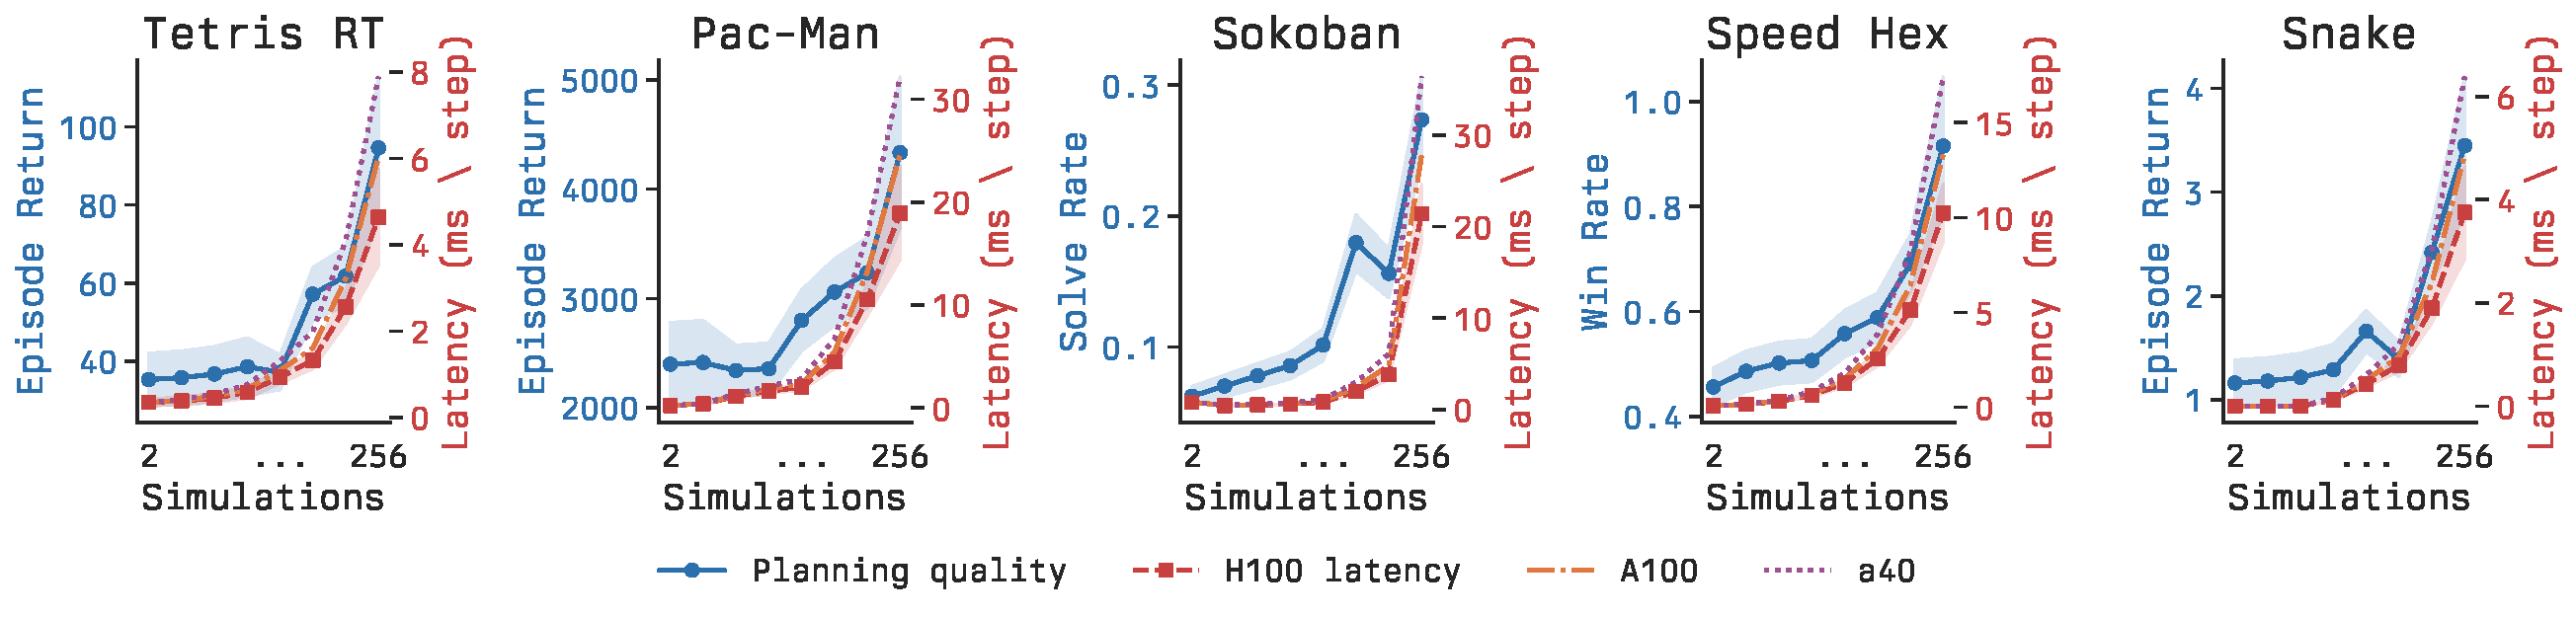
\includegraphics[width=\linewidth]{figures/scaling.pdf}
  \caption{Planning quality and real-time inference latency co-scale with simulation
    count across all five environments.
    \emph{Blue solid}: performance (episode return, solve rate, or win rate).
    \emph{Dashed lines}: per-step inference latency on H100,
    A100, and A40.
    Shaded band shows $\pm$SE.}
  \label{fig:scaling}
\end{figure}

This joint scaling makes the allocation problem tractable. We do not need to learn
\emph{how} to plan, the planner handles that, only \emph{when} the additional quality
gain is worth the additional real-time cost.

\subsection{Variable-duration meta-decisions}

We formalize planning-depth selection as a Semi-Markov Decision Process (SMDP).
At each meta-step the gating policy $\pigate(K \mid s_t)$ selects a depth
$K_t \in \Kset$.
The agent executes $K_t{-}1$ committed actions followed by the planner's chosen
action, accumulating rewards over all $K_t$ steps:
\begin{equation}
  R_t = \sum_{k=0}^{K_t - 1} r_{t+k}.
  \label{eq:meta_reward}
\end{equation}
The same formulation covers clock environments: the $K_t{-}1$ committed actions
are no-ops that contribute zero reward, so $R_t$ reduces to the reward of the
planner's chosen action while $\gamma^{K_t}$ in equation~\eqref{eq:smdp} still
discounts the elapsed clock cost.
The next meta-state is $s_{t + K_t}$, and the Bellman target uses a per-meta-step
discount of $\gamma^{K_t}$:
\begin{equation}
  V(s_t) = \mathbb{E}_{K_t \sim \pigate}\!\left[R_t + \gamma^{K_t} V(s_{t+K_t})\right].
  \label{eq:smdp}
\end{equation}
We adapt Generalized Advantage Estimation~\cite{schulman2015high} to carry the
per-step discount factor $\gamma^{K_t}$ through the advantage computation.

\paragraph{Reward formulation.}
We use the raw, unnormalized meta-reward~\eqref{eq:meta_reward}.
Normalizing by $K$ or discounting the reward itself (rather than only the future value)
creates an implicit bias toward $K{=}1$: longer options must accumulate proportionally
more reward to be competitive, regardless of whether deeper planning actually earns
more.
Raw reward lets the policy discover when deeper planning is worth more. \am{will double check on the reasoning on this, maybe can introduce small formalism in the appendix for this}

\subsection{What the gating policy observes}

The gating policy takes three inputs at each meta-step:
(1) the raw game grid,
(2) the planner's intermediate spatial features extracted from its frozen trunk
(a global summary of what the planner infers about the current position), and
(3) the planner's scalar value estimate $V(s_t)$.
In clock environments the observation also includes the remaining time budget.
Together these give the gating policy both a direct view of the board and a compressed
summary of the planner's own confidence, without requiring any access to the planner's
internals beyond a single forward pass.
A lightweight network processes these inputs and produces a distribution over $K$ and
a baseline value for training.
All architecture and training details are in Appendix~\ref{app:implementation}.

\subsection{Training}

The gating policy is trained with PPO~\cite{schulman2017proximal} on top of the
frozen planner.
Rollouts are collected over full episodes; SMDP-adapted advantages are computed before
each round of policy updates.
Only the gating network is updated; the planner receives no gradient.


% =============================================================================
\section{Experiments}
\label{sec:experiments}
% =============================================================================

\subsection{Setup}

\paragraph{Environments.}
We evaluate across five environments spanning both mechanisms (Table~\ref{tab:envs}).

\begin{table}[h]
  \centering
  \caption{Evaluation environments.}
  \label{tab:envs}
  \small
  \begin{tabular}{lll}
    \toprule
    Environment & Mechanism & Sim options \\
    \midrule
    \multicolumn{3}{l}{\textit{Committed-action}} \\[2pt]
    Pac-Man (Jumanji) & Committed-action & 32, 64, 96, 128 \\
    Real-Time Tetris  & Committed-action & 32, 64, 96, 128 \\
    Snake             & Committed-action & \{1, 2, 4\}  \emph{(training)} \\[4pt]
    \multicolumn{3}{l}{\textit{Clock}} \\[2pt]
    Speed Hex (11$\times$11) & Explicit clock & 2, 8, 32, 128 \\
    Timed Sokoban & Explicit clock & 2, 8, 32, 64 \\
    \bottomrule
  \end{tabular}
\end{table}

\paragraph{Baselines.}
For committed-action environments we compare against: \emph{always-$K$} policies for
each $K \in \Kset$; and a \emph{random} policy selecting $K$ uniformly at each
meta-step.
For speed environments we additionally compare against \emph{greedy} (always use
maximum simulations) and \emph{midpeak} (a bell-curve allocation that concentrates
compute at the critical mid-game, a common heuristic in game engines \cite{baier2016time, huang2010timemanagement}).

\am{need to add to appendix that bell curve is tuned per budget that we eval against}

\paragraph{Base planner.}
For committed-action environments we use an AlphaZero checkpoint trained without
action delay ($K{=}1$) as the frozen base.
Cross-evaluation across checkpoints trained at each $K$ shows this checkpoint
dominates at all evaluation depths (Appendix~\ref{app:cross_eval}).

\paragraph{Evaluation protocol.}
All results are averaged over 100 independent episode seeds; we report mean $\pm$ standard error.

\subsection{Main results}

\begin{figure}[t]
  \centering
  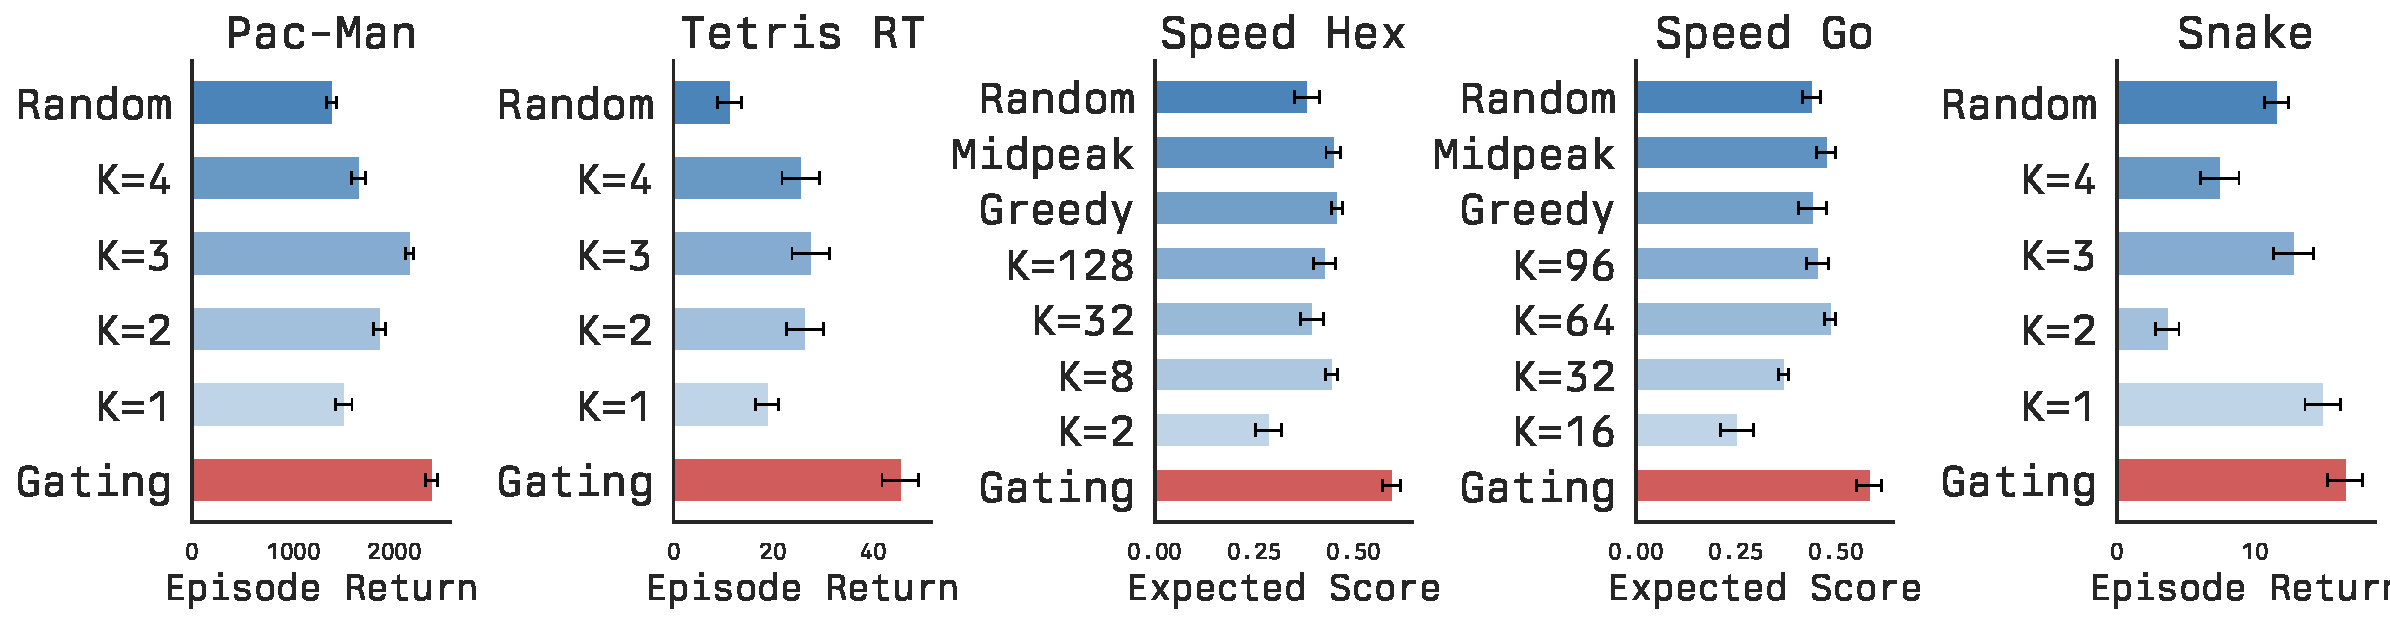
\includegraphics[width=\linewidth]{figures/main_results_horizontal.pdf}
  \caption{Main results (mean $\pm$\,SE, 100 episodes).
    Colored bars: gating policy (ours); blue bars: baselines.
    Tetris RT uses the RT\_KT variant (MCTS-step committed actions). \am{we need to talk about how to present budget results, we can say we have per budget results in appendix. We sample budgets we didn't train on, and have a budget by budget analysis in appendix. 5 budgets}}
  \label{fig:main_results}
\end{figure}

The gating policy outperforms every fixed-budget baseline across all environments.
In Pac-Man the best fixed policy ($K{=}3$, 96 sims/step) scores 2149; the gating policy
reaches 2370 ($+10.3\%$) using only ${\approx}49$ simulations per frame on average.
In real-time Tetris the best fixed policy ($K{=}3$) scores 27.6; the gating policy
reaches 45.6 ($+65\%$) using a bimodal strategy described below.
The random baseline falls well below every fixed-$K$ policy in both environments,
confirming that \emph{when} to allocate compute matters as much as how much.

In Snake the best fixed policy ($K{=}1$) scores 14.91; the gating policy reaches 16.54 ($+10.9\%$) by predominantly reacting quickly ($K{=}1$, 81.6\% of steps) while selectively invoking deeper planning as the board becomes constrained.

\subsection{Learned depth distribution}

In Pac-Man the policy adopts a near-binary strategy: $K{=}1$ (51.9\%) for most steps
and $K{=}2$ (44.9\%) for demanding ones, with $K{=}4$ (3.1\%) reserved for rare
extremes, averaging ${\approx}49$ simulations per frame, well below the 96 of the
best fixed policy.
In Tetris the distribution is strongly bimodal: $K{=}4$ (51.7\%), $K{=}1$ (28.1\%),
$K{=}2$ (20.2\%), with $K{=}3$ never selected (0\%).
The policy has effectively learned a sharp binary. It learns to react immediately on easy boards and plan maximally on critical ones, with $K{=}2$ handling moderate cases.
In Snake, $K{=}1$ dominates throughout ($81.6\%$) with $K{=}2$ handling moderate cases ($15.2\%$) and $K{=}3$ rising as the snake elongates ($3.2\%$ overall); $K{=}4$ is never selected ($0\%$), mirroring the $K{=}3$ avoidance in Tetris.
Figure~\ref{fig:strategy} shows how the allocation shifts over the course of an episode.

\subsection{What triggers deeper planning?}

Across the environments, the gating policy concentrates compute in high-stakes states:
situations where the consequence of a suboptimal action is large and additional search
depth is most likely to change the decision.

\paragraph{Pac-Man}

The clearest signal in Pac-Man is ghost proximity: the policy prefers $K{=}1$ when the
nearest ghost is far away, shifts toward $K{=}2$ as the threat closes in, and reaches
for $K{=}4$ at extreme proximity. When ghosts are frightened the threat evaporates, and
the policy reduces planning depth accordingly.

\paragraph{Tetris}

Board density is the dominant feature in Tetris.
$K{=}1$ is selected almost exclusively on near-empty boards
(fill $\approx 0.05$, stack $\approx 3.5$ rows) where any reasonable placement is
acceptable.
$K{=}2$ and $K{=}4$ are selected on dense boards (fill $\approx 0.25$--$0.32$,
stacks $\approx 12$ rows) where placement precision is consequential.
$K{=}3$ is never used ($0\%$), producing the bimodal ``react or plan deeply'' strategy
visible in Figure~\ref{fig:strategy}.
Piece type also modulates depth: the Z-piece ($\bar{K}{=}2.98{\scriptstyle\pm0.04}$)
and O- and T-pieces ($\bar{K}{=}2.88{\scriptstyle\pm0.04}$) receive the most
deliberation, while the J-piece ($\bar{K}{=}2.66{\scriptstyle\pm0.04}$) receives the
least, reflecting differences in placement geometry and expected outcome variance.

\paragraph{Snake}

Spatial constraint---not goal difficulty---is the primary trigger, and $K{=}2$
and $K{=}3$ respond to \emph{different} aspects of it.
$K{=}1$ dominates on open boards: mean snake length $8.76{\scriptstyle\pm0.04}$,
flood-fill reachability $134.7$ cells (93.5\% of the $12{\times}12$ grid),
local body density $26.9\%$ in the $3{\times}3$ neighbourhood, and $3.27$ valid moves.
$K{=}3$ activates when space is scarce: length $20.42{\scriptstyle\pm0.25}$,
reachability drops to $120.4$ cells (${\downarrow}10.5\%$),
local density rises to $33.6\%$, and only $2.85$ valid moves remain---the fewest
of any $K$.
Crucially, $K{=}3$'s mean fruit distance ($7.81$) is \emph{similar} to $K{=}1$'s
($8.09$), confirming that the trigger is topological crowding, not goal difficulty.
$K{=}2$ occupies a distinct niche: it fires on the most open boards (most valid
moves, $3.45$; lowest local density, $23.5\%$) but with the \emph{farthest} fruit
($9.96$ cells).
The policy has learned to reach for one extra planning step specifically when
navigating toward a distant goal on an uncrowded board---a separate concern from
spatial danger.
The post-eating transition reinforces the picture: immediately after consuming
fruit (1{,}546 events, snake just grew longer), $K{=}3$ usage spikes from
$3.2\%$ to $13.5\%$ ($4{\times}$), showing the policy responds in real time to
body-growth events as a prospective spatial risk signal.

\begin{figure}[t]
  \centering
  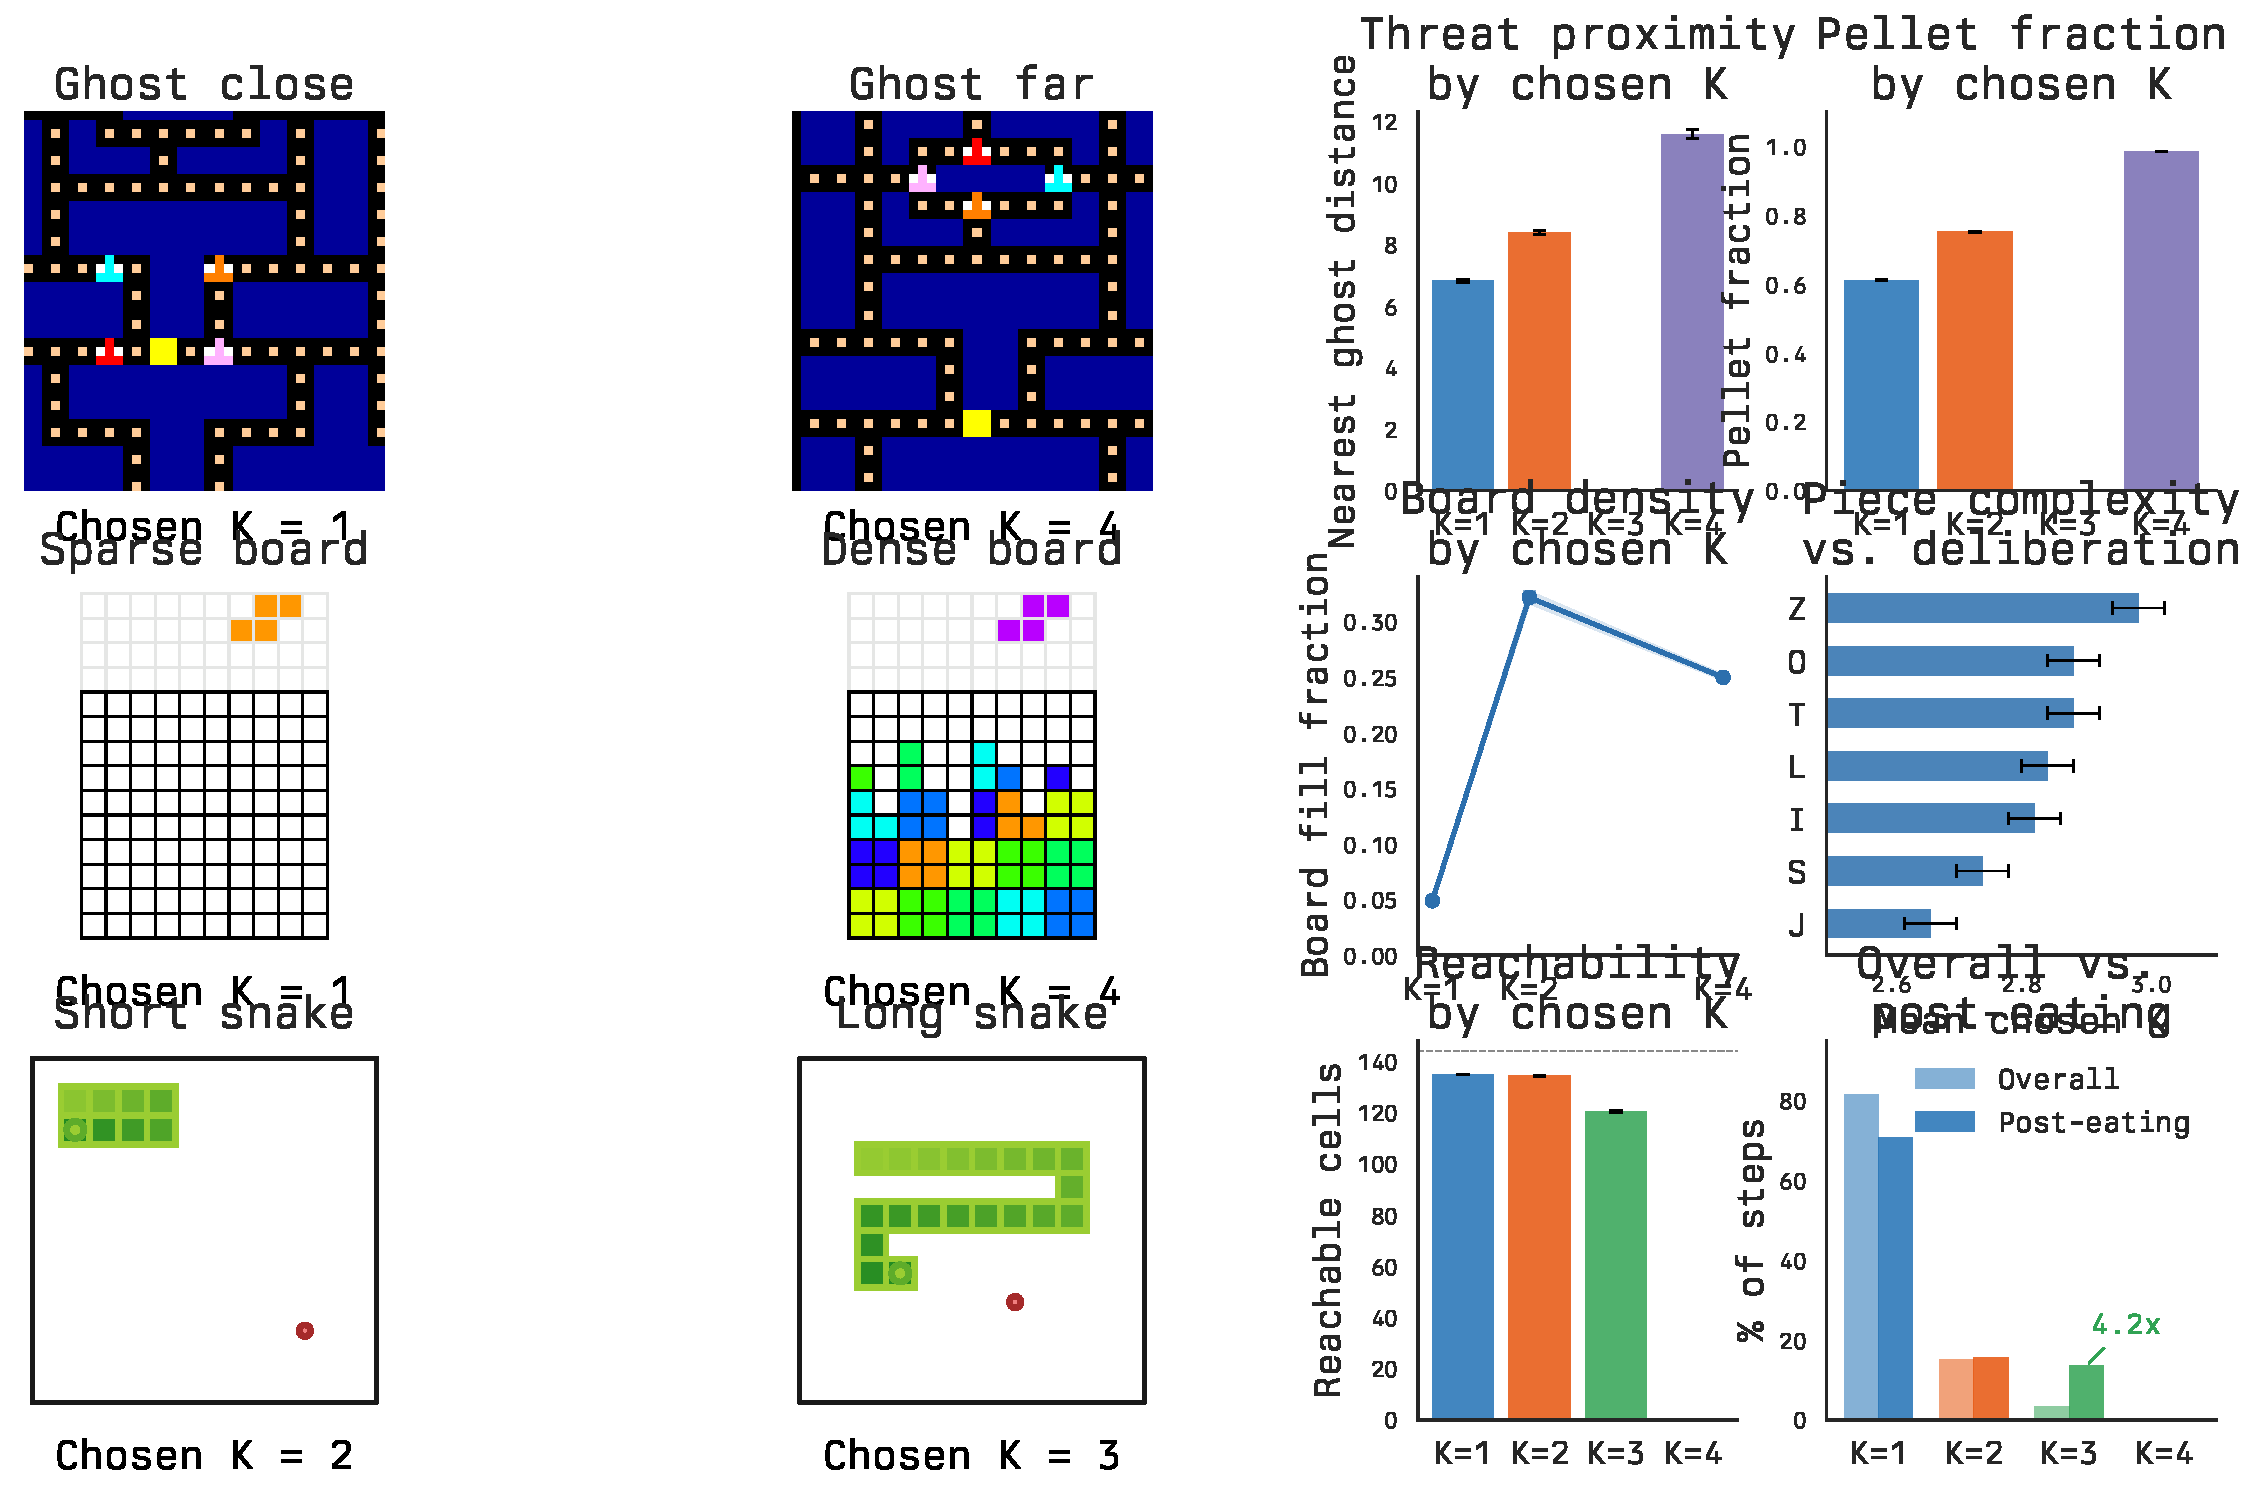
\includegraphics[width=\linewidth]{figures/interpretability_combined.pdf}
  \caption{Interpretability: state features conditioned on chosen depth $K$
    (mean $\pm$\,1\,SE, 100 episodes).
    \emph{Top:} In Pac-Man, ghost-far states elicit $K{=}4$; ghost-close states
    elicit $K{=}1$; rightmost panel shows mean nearest-ghost distance by chosen $K$.
    \emph{Middle:} In Tetris RT, a sparse board elicits $K{=}1$; a dense board
    elicits $K{=}4$; center panel shows board fill by chosen $K$
    ($K{=}3$ never selected); right panel shows mean chosen $K$ by piece type.
    \emph{Bottom:} In Snake, flood-fill reachability (left) and local $3{\times}3$
    body density (center) by chosen $K$: $K{=}3$ triggers on the most constrained
    boards (reachability $120.4$ vs.\ $134.7$ for $K{=}1$; $K{=}4$ never selected).
    Right: $K$ distribution overall (faded) vs.\ immediately after eating fruit
    (solid); $K{=}3$ spikes $4{\times}$ ($3.2\%{\to}13.5\%$) when the snake has
    just grown, signalling prospective spatial risk.}
  \label{fig:interpretability}
\end{figure}

\paragraph{Speed environments.}
\todo{Describe what features trigger more thinking in speed Hex / Sokoban: remaining
clock, board contestedness, etc.}

\subsection{Planning depth allocation over episode time}

\begin{figure}[t]
  \centering
  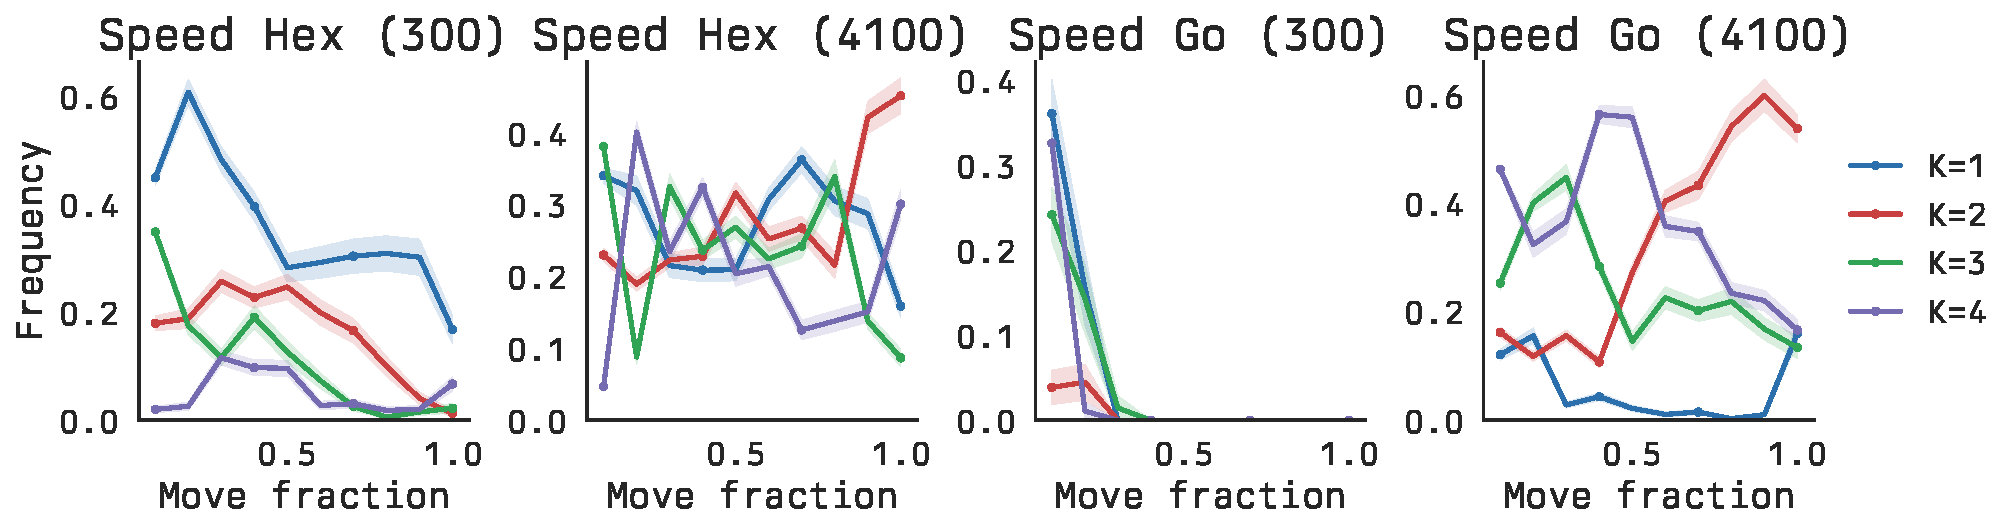
\includegraphics[width=\linewidth]{figures/strategy.pdf}
  \caption{Planning depth frequency over normalized episode time (10 equal bins).
    Lines: fraction of steps at which each depth or sim-count option was chosen.
    Pac-Man, Tetris RT, Sokoban, and Snake: $K \in \{1,2,3,4\}$; Speed Hex: sim counts
    $\{2,8,32,128\}$ (same line colors).
    Shared legend shown on the right; line styles consistent across all panels.}
  \label{fig:strategy}
\end{figure}


% =============================================================================
\section{Real-Time Deployment}
\label{sec:deployment}
% =============================================================================

We validate the committed-action framework in a true two-GPU real-time setup across
three committed-action environments: real-time Tetris, Pac-Man, and Snake.
One GPU runs the environment and executes committed actions continuously; a second GPU
runs the MCTS planner.
At each meta-decision the current game state is transferred to the planning GPU, which
begins search while the environment GPU keeps the game moving with committed actions.
When planning finishes, after $K \times 32$ simulations, the result is applied at
the next environment step.

Figure~\ref{fig:deployment} summarizes 45 measured deployments:
3 environments $\times$ 3 GPU classes $\times$ 5 frame rates (8--12\,FPS).
The asynchronous execution pattern itself is unchanged from training: a $K{=}4$
meta-step at 9\,FPS spans four 111\,ms frames, while reflex actions keep the
environment moving and MCTS finishes asynchronously on the second GPU.

The latency measurements show that the deployment remains comfortably in-budget on
modern accelerators for most of this operating range.
At 9\,FPS in Tetris, where the $K{=}4$ budget is 444\,ms, H100 latency is
$123.9$\,ms on average (p95 $207.6$\,ms; $0.014\%$ miss rate), A100 is
$186.3$\,ms (p95 $312.1$\,ms; $0.014\%$), and A40 is $197.7$\,ms
(p95 $339.0$\,ms; $0.046\%$).
Across all tested FPS values, H100 remains extremely reliable in all three
environments, and A100 remains near-perfect in Tetris and Snake.
The main failures arise exactly where the budget becomes tight.
In Tetris on A40, p95 slack shrinks from $+162.2$\,ms at 8\,FPS to $-4.1$\,ms
at 12\,FPS, and the miss rate jumps from $0.046\%$ to $50.669\%$.
Pac-Man is the most latency-sensitive environment overall: at 12\,FPS, miss rate
reaches $30.369\%$ on A100 and $13.073\%$ on A40, whereas Snake remains negligible
throughout ($\le 0.005\%$ on all hardware/FPS settings tested).

The return results show that simulation-to-deployment transfer remains strong despite
these hardware and frame-rate changes.
At 9\,FPS, deployed Tetris return is $41.4 \pm 4.2$ on H100 versus
$45.6 \pm 3.7$ in simulation, $46.2 \pm 4.5$ on A100, and $42.7 \pm 7.7$ on A40.
Pac-Man remains close to its simulated return of $2370 \pm 59$ on H100
($2287.4 \pm 55.2$) and A40 ($2368.3 \pm 116.0$), with a larger but still
functional drop on A100 ($2117.2 \pm 64.3$).
Snake is similarly stable: simulation return is $16.54 \pm 1.26$, compared to
$15.0 \pm 0.6$ on H100, $15.9 \pm 0.6$ on A100, and $14.9 \pm 1.2$ on A40.
The learned depth distributions also transfer cleanly. In Tetris, for example,
the deployed policy remains strongly bimodal:
$K{=}4$: $52.8\%$, $K{=}1$: $29.1\%$, $K{=}2$: $18.1\%$, $K{=}3$: $0\%$
on H100 at 9\,FPS, versus $51.7\%$, $28.1\%$, $20.2\%$, $0\%$ in simulation.

This result demonstrates a key property of the committed-action training protocol.
Because training simulates the planning delay by actually executing committed actions
in the environment, the learned policy requires no modification for deployment.
The separation between environment and planner is already the right abstraction.
The Real-Time RL framework~\citep{ramstedt2019rtrl} fixes the computation budget to
exactly one timestep via a 1-step delay RTMDP state augmentation---adequate for
lightweight policies but insufficient for variable-depth MCTS spanning
$K \in \{1,\ldots,4\}$ frames, where a naive extension would require carrying $K$
stale actions in the state.
Appendix~\ref{app:deployment_details} gives the full environment-by-FPS-by-GPU
deployment breakdown, while Appendix~\ref{app:rtrl_smdp} gives a formal account
of how committed-action training relates to the RTMDP and SMDP formalisms and why
it avoids this state-augmentation problem entirely.

\begin{figure}[h]
  \centering
  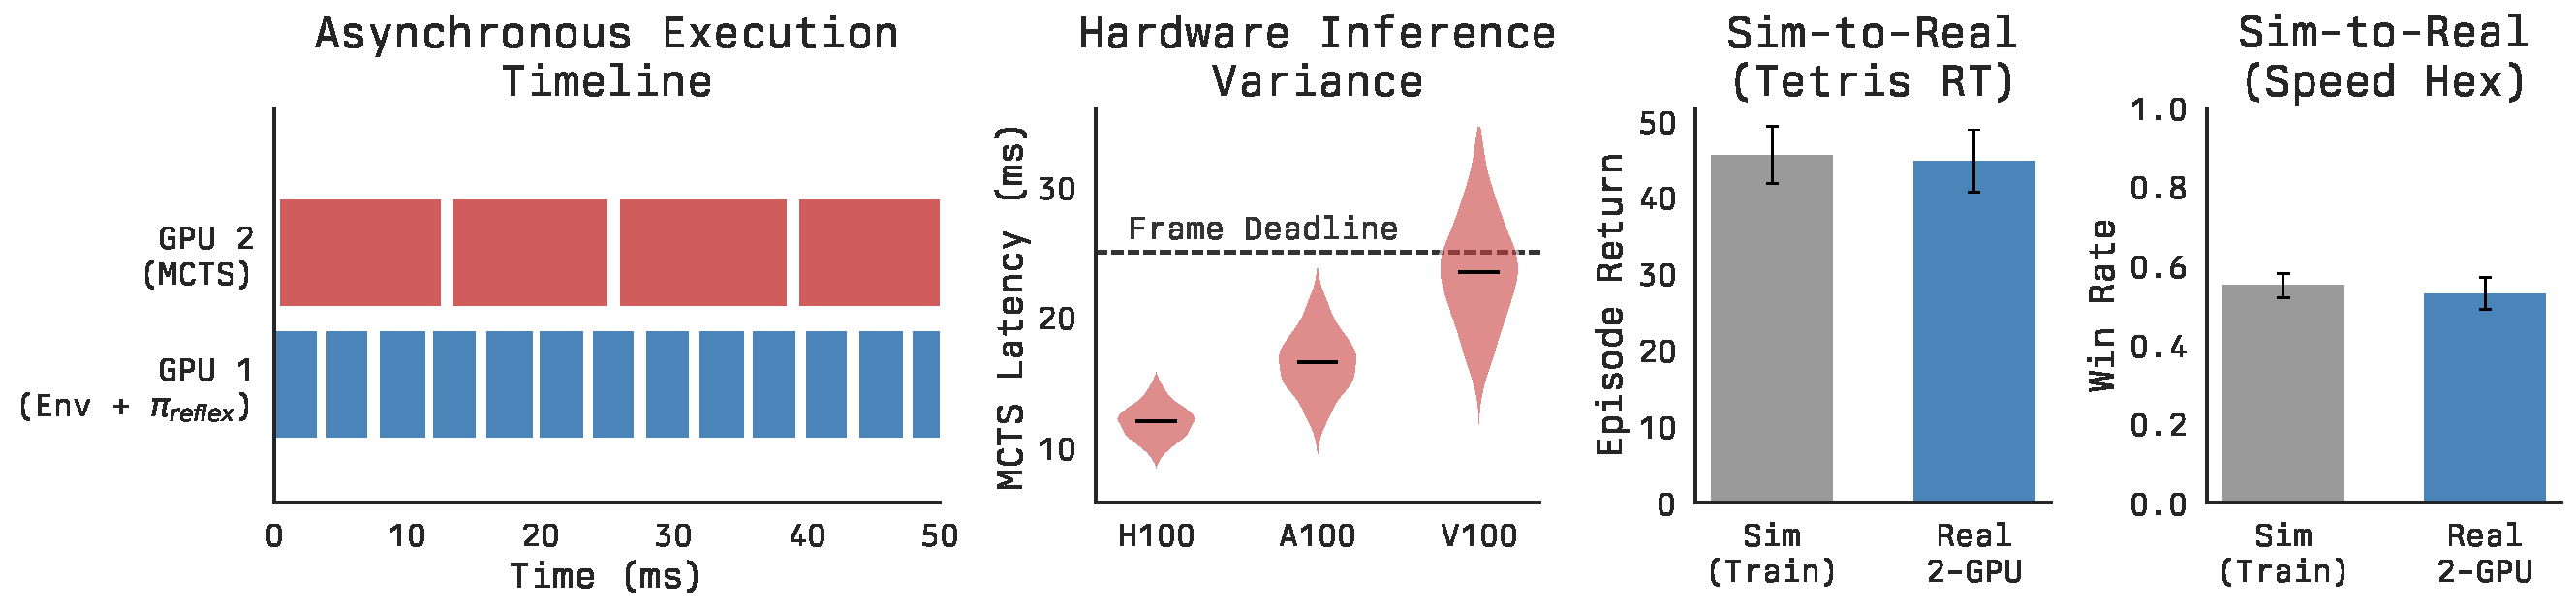
\includegraphics[width=\linewidth]{figures/deployment.pdf}
  \caption{Validation of the real-time, asynchronous 2-GPU deployment.
    \emph{Left:} Timeline of execution showing the environment and committed-action
    policy ($\pi_{reflex}$) running at 9\,FPS on GPU~0 while the MCTS planner
    runs asynchronously on GPU~1.
    A K{=}4 meta-step spans 4 frames (444\,ms); MCTS finishes at $\approx$200\,ms,
    leaving large slack before the deadline.
    \emph{Center-left:} Measured MCTS latency distributions aggregated across
    Tetris, Pac-Man, and Snake for H100, A100, and A40 deployments.
    \emph{Center-right:} Average deadline miss rate across environments, showing
    H100 remains near-zero overall while A40 incurs the largest reliability cost.
    \emph{Right:} Sim-to-real return normalized to simulation (simulation $=100\%$)
    at 9\,FPS.
    Transfer remains strong across all three environments, even as hardware
    reliability diverges near the deadline boundary. Full per-environment,
    per-FPS, per-GPU results appear in Appendix~\ref{app:deployment_details}.}
  \label{fig:deployment}
\end{figure}

% =============================================================================
\section{Discussion}
% =============================================================================

\paragraph{Learned value of computation.}
The gating policy is learning a value-of-computation function~\cite{russell1991right}
from experience.
At each state it implicitly asks, is the expected improvement from deeper planning
worth the additional real-time cost?
The answer is state-dependent and interpretable. Higher when the board is dense, when
threats are close, and when the piece type makes placement precision consequential.
The fact that this function can be learned end-to-end, without explicit cost modeling
or hand-designed metareasoning rules, is itself a finding: VoC reasoning emerges from
standard RL training when the cost structure is embedded in the environment.

\paragraph{A unified framework.}
The committed-action and clock mechanisms are two realizations of the same underlying
principle that planning is cost-aware by construction.
In committed-action environments, cost-awareness is baked into the MCTS tree itself,
which simulates committed-action steps and therefore searches over the exact future
the agent will experience.
In clock environments, cost-awareness is baked into the network's value estimates,
which are trained on clock-augmented observations and therefore price in remaining
budget.
The gating policy can exploit both signals using the same learning algorithm.

\paragraph{Deployment as a test of training fidelity.}
The two-GPU deployment result is not merely an engineering demonstration.
It shows that the committed-action abstraction, where K-1 reflex actions fill
the planning delay in simulation, accurately models the dynamics of true asynchronous
execution.
An agent trained under this abstraction generalizes immediately to hardware-separated
deployment, suggesting the abstraction captures the essential real-time structure.

\paragraph{Limitations.}
The gating policy trains on top of a fixed base planner; joint optimization of the
two is an open problem.
We study a discrete depth set $K \in \Kset$; continuous compute allocation is a
natural extension.
Our environments are either simulation-based or played at controlled speeds; extending
to physical real-time settings with uncontrolled latency would require adaptive
calibration of the timing model.


% =============================================================================
\section{Conclusion}
% =============================================================================

We studied the problem of planning in real-time reinforcement learning, where the
cost of deliberation is paid in game outcomes rather than wall-clock seconds.
Planning quality and real-time inference cost co-scale with simulation depth, making
adaptive depth selection the natural lever for performance.
A lightweight gating policy, trained via RL on top of a frozen planner, learns to
invest computation proportionally to situational state complexity, more for dense
boards and high-stakes decisions, less for easy ones.
Across five environments spanning two real-time mechanisms, the gating policy
consistently outperforms every fixed-budget baseline while using less average compute.
We believe that adaptive, state-conditioned compute allocation is an important and
underexplored axis for making planning-based RL systems both more capable and
more resource-efficient in real-time settings.


\begin{ack}
\todo{Acknowledgments, funding disclosure, and competing interests.}
\end{ack}


% =============================================================================
% =============================================================================

\bibliographystyle{plainnat}
\bibliography{refs}


%%%%%%%%%%%%%%%%%%%%%%%%%%%%%%%%%%%%%%%%%%%%%%%%%%%%%%%%%%%%
\appendix

\section{AlphaZero and MCTS}
\label{app:az_primer}

This section answers common questions about the planning infrastructure used in this
paper. It targets readers familiar with deep RL but not with tree-search methods.

\textbf{What does ``running a simulation'' mean in MCTS?}

A \emph{simulation} (also called a \emph{playout}) is one traversal of the search tree
from the root node (the current observed state) to a leaf, followed by a backup of
the resulting value estimate up to the root.
Each traversal selects edges greedily according to the PUCT rule:
\[
  a^* = \arg\max_a \Bigl[Q(s,a)
        + c \cdot \pi_\theta(a|s)
          \cdot \frac{\sqrt{N(s)}}{1+N(s,a)}\Bigr],
\]
where $Q(s,a)$ is the empirical mean value of subtree $a$,
$\pi_\theta(a|s)$ is the network's prior over actions,
$N(s)$ is the total visit count of node $s$,
and $N(s,a)$ is the visit count of edge $(s,a)$.
Repeated simulations concentrate visits on high-value, high-prior subtrees while
continuing to explore less-visited ones.
After $n$ simulations the recommended action is the \emph{most-visited} child of
the root.

\textbf{How is the final action selected?}

At evaluation time the agent picks the most-visited root child.
During training, the visit-count distribution
$\hat{\pi}(a) \propto N(s_0,a)^{1/\tau}$
(temperature $\tau > 0$) is recorded and used as a \emph{search target}:
the network is updated to predict $\hat{\pi}$ at state $s_0$.
This is the expert-iteration loop as search produces a better-than-raw-policy
distribution, and the network learns to imitate it, improving its prior for
future searches.


\textbf{What is the difference between AlphaZero and MuZero?}

\textbf{AlphaZero}~\cite{silver2018general} requires a \emph{perfect simulator}:
given state $s$ and action $a$, the simulator returns the exact next state $s'$.
MCTS is run entirely inside this simulator; the network supplies priors and value
estimates but never models transitions.

\textbf{MuZero}~\cite{schrittwieser2020muzero} replaces the perfect simulator with a
\emph{learned latent-space dynamics model}.
Transitions during search are predicted by a network rather than a ground-truth
engine, so MuZero can plan in environments without a simulator (e.g.\ Atari frames).

All environments in this paper expose a JAX-native step function, so we use the
AlphaZero paradigm: ground-truth transitions, no learned dynamics.

\textbf{AlphaZero was designed for two-player zero-sum games. How does it transfer to single-agent settings?}

The core loop is \emph{expert iteration}~\cite{anthony2017thinking},
shown in Algorithm~\ref{alg:expert_iter}.
The value head uses a bootstrapped return instead of a zero-sum game outcome;
otherwise the algorithm is identical to two-player AlphaZero.

\begin{algorithm}[h]
\caption{Single-agent AlphaZero via Expert Iteration}
\label{alg:expert_iter}
\begin{algorithmic}[1]
\Require Network $f_\theta = (\pi_\theta, v_\theta)$, environment $\mathcal{E}$,
         simulations per step $n$, replay buffer $\mathcal{B}$
\Repeat
  \State $\mathcal{D} \leftarrow \{\}$ \Comment{episode data buffer}
  \State $s_0 \leftarrow \mathcal{E}.\text{reset}()$
  \For{$t = 0, 1, \ldots, T-1$}                     \Comment{\textbf{Act}}
    \State Run $n$ MCTS simulations from $s_t$ using $f_\theta$
    \State $\hat{\pi}_t(a) \propto N(s_t, a)^{1/\tau}$ \Comment{visit-count policy}
    \State $a_t \sim \hat{\pi}_t$;\quad $s_{t+1} \leftarrow \mathcal{E}.\text{step}(a_t)$
    \State $\mathcal{D} \leftarrow \mathcal{D} \cup \{(s_t,\, \hat{\pi}_t)\}$
  \EndFor
  \State Compute returns $z_t = \sum_{k \geq 0} \gamma^k r_{t+k}$ for each $t$ \Comment{\textbf{Store}}
  \State $\mathcal{B} \leftarrow \mathcal{B} \cup \{(s_t, \hat{\pi}_t, z_t)\}_{t=0}^{T-1}$
  \State Sample mini-batch from $\mathcal{B}$                     \Comment{\textbf{Learn}}
  \State $\mathcal{L}(\theta) =
    \displaystyle\frac{1}{|\mathcal{B}|}\sum_{(s,\hat{\pi},z)\in\mathcal{B}}
    \Bigl[\bigl(v_\theta(s) - z\bigr)^2
          - \hat{\pi}^\top \log \pi_\theta(s)\Bigr]$
  \State $\theta \leftarrow \theta - \alpha\,\nabla_\theta\,\mathcal{L}(\theta)$
\Until{convergence}
\end{algorithmic}
\end{algorithm}


\textbf{MCTS sounds inherently sequential. How do you run it efficiently at the scale needed for RL training?}

Naively each MCTS simulation depends on the previous one (via the updated $Q$ and $N$
tables), which conflicts with JAX's strength: massive data-parallel operations.
We exploit two levels of parallelism.

\textbf{Environment-level parallelism.}
We maintain a batch of $E$ independent environment instances (32 in our experiments).
Each instance has its own search tree; all $E$ leaf nodes are evaluated in a
\emph{single batched forward pass} of the neural network, which is the GPU/TPU
bottleneck.

\textbf{Intra-tree simulation loop via \texttt{jax.lax.scan}.}
Within each tree the $n$ simulations are unrolled as a \texttt{scan}.
Each iteration: (1) traverse all $E$ trees to their current leaf using PUCT
(parallelised over $E$), (2) batch-evaluate the $E$ leaves in one network call,
(3) back-propagate values.
Because JAX traces the full scan at compile time, the tree-update logic is fused
into a single XLA kernel with zero Python-level iteration overhead at runtime.

The result is that all $n$ simulations across all $E$ environments are compiled
into a single \texttt{jit}-ted function that runs entirely on the accelerator,
with one network forward pass per simulation step and no host-device transfers
during rollout.


\section{Environment Details}
\label{app:envs}

\subsection{Real-time Tetris}
Every call to \texttt{env.step(action)} advances the falling piece by one gravity row
(gravity tick).
The action set has six elements:
\begin{itemize}[nosep]
  \item \textbf{Left / Right}: translate the falling piece one column in the respective
    direction.
  \item \textbf{Rotate-CW / Rotate-CCW}: rotate the piece $90°$ clockwise or
    counter-clockwise.
  \item \textbf{Hard-drop}: instantly translate the piece to the lowest valid row and
    lock it; a new piece spawns immediately.
  \item \textbf{Forward} (default): no horizontal movement; the piece descends one row
    by gravity.
\end{itemize}
A piece locks when gravity would place it in an occupied cell; completed rows are then
cleared and scored.
The episode ends on board top-out (a newly spawned piece immediately collides) or after
2000 gravity ticks.

\subsection{Committed-action execution}
\label{app:committed_action}

During the $K{-}1$ delay steps while the MCTS planner is running, the agent must
continue acting in the environment.
We evaluate two variants.

\textbf{RT (logit)} uses the argmax of the base model's raw policy logits as the
committed action at each delay step---a single inexpensive forward pass per step.

\textbf{RT\_KT (MCTS-step)} uses one full MCTS step (a small tree search) as the
committed action at each delay step, producing higher-quality interim decisions at
the cost of additional compute.
This variant is more consistent with Pac-Man, where the committed (blueprint) policy
leverages the planner's tree internally.
All Tetris results reported in the main paper use the RT\_KT variant.

In both variants the MCTS recurrent function simulates the same $K{-}1$ committed-action
steps on each edge of the main search tree, ensuring that search is conducted over the
exact future the agent will experience.

\subsection{Speed Hex}
Speed Hex is built on the pgx Hex library (11$\times$11 board).
Each player begins with $T = 300$ clock ticks; time spent planning is deducted after
each move.
MCTS search uses board-only dynamics (no clock deduction during simulation), but the
observation (and therefore the network's value estimates) includes the remaining
clock for both players.
The gating policy is a GRU network that maintains hidden state across moves within an
episode, allowing it to track game progression and clock pressure jointly.


\section{Simulation Option Calibration for Clock Environments}
\label{app:sim_calibration}

For committed-action environments, the equal-budget constraint (32 sims/frame) naturally
produces meaningful option spacing.
For clock environments this constraint does not apply, so we select simulation options
by examining two curves simultaneously: planning quality (win rate or return) vs.\
simulation count, and inference latency vs.\ simulation count.

An option is \emph{useful} if it is distinguishable from its neighbors on both dimensions:
adding more simulations should noticeably improve play \emph{and} noticeably increase
latency.
Options that are close in both cost and quality give the gating policy nothing to learn;
options that differ in cost but not quality waste planning budget.

For speed Hex we found that options $\{2, 8, 32, 128\}$ satisfy this criterion across
the relevant range of clock settings.
\todo{Insert calibration curves: win rate vs.\ sims, latency vs.\ sims, with chosen
options marked.}


\section{Cross-Evaluation and Base Model Selection}
\label{app:cross_eval}

We trained four AlphaZero checkpoints at delay depths $K \in \Kset$ and evaluated
all 16 (train-$K$, eval-$K$) combinations.

\todo{Table: 4$\times$4 cross-evaluation matrix.}

The $K{=}1$-trained checkpoint dominates at every evaluation depth.
Two factors compound: $K{=}1$ training is causally clean (no delay confounds the
value function), and committed actions during delay steps are drawn from the base
model's policy---a stronger base produces better committed actions and therefore better
states when the MCTS action fires.
We use the $K{=}1$ checkpoint as the frozen base for all committed-action experiments.


\section{Implementation Details}
\label{app:implementation}

\subsection{Gating network architecture}

\textbf{Spatial branch.}
The game grid is processed by a $1{\times}1$ convolution lifting to 64 channels,
followed by three residual blocks with Layer Normalization and global average pooling
to a 64-dimensional spatial representation.
Layer Normalization is used because the gating policy operates on a single environment
instance per rollout step, making batch statistics undefined.

\textbf{Time / clock embedding.}
For committed-action environments, the normalized step count is encoded as a 2-vector
and projected through a small MLP before being added to the spatial features.
For clock environments, the remaining clock fraction is similarly embedded and added.

\textbf{Fusion and heads.}
The spatial representation (64-dim), planner trunk features (128-dim), and planner
value (1-dim) are concatenated and passed through dual MLP heads: a policy head
producing logits over $K$, and a value head producing a scalar baseline.

\textbf{Speed Hex gating network.}
Uses a GRU backbone rather than a feedforward network, maintaining a recurrent hidden
state across moves within each game to track temporal context.

\subsection{Training hyperparameters}

\begin{table}[h]
  \centering
  \caption{PPO hyperparameters for committed-action environments.}
  \label{tab:hparams}
  \begin{tabular}{lcc}
    \toprule
    Hyperparameter & Pac-Man & Tetris RT \\
    \midrule
    Num.\ parallel envs     & 32   & 32   \\
    Meta-steps per rollout  & 384  & 384  \\
    PPO epochs per rollout  & 4    & 4    \\
    Num.\ mini-batches      & 16   & 16   \\
    Meta-reward mode        & raw  & raw  \\
    Discount $\gamma$       & 0.99 & 0.99 \\
    GAE $\lambda$           & 0.95 & 0.95 \\
    PPO clip $\epsilon$     & 0.2  & 0.2  \\
    Entropy coefficient     & 0.01 & 0.01 \\
    Learning rate           & 3e-4 & 3e-4 \\
    Sim options             & 32, 64, 96, 128 & 32, 64, 96, 128 \\
    \bottomrule
  \end{tabular}
\end{table}


\section{Timing Results}
\label{app:timing}

Full timing table for all environments and $K$ options:
\todo{Insert complete latency / FPS table once measurements are collected.}


\section{Detailed Two-GPU Deployment Breakdown}
\label{app:deployment_details}

We ran the full asynchronous deployment grid for all 45 settings:
3 environments (Tetris, Pac-Man, Snake) $\times$ 3 GPUs (H100, A100, A40)
$\times$ 5 frame rates (8--12\,FPS).
Figure~\ref{fig:deployment_appendix} gives the complete breakdown by environment,
GPU, and FPS for return, deadline miss rate, and p95 slack to deadline.

Several patterns are clear.
First, H100 is consistently reliable across the entire tested range.
In Tetris its miss rate stays at $0.014\%$ for all FPS values, with p95 slack
remaining positive from $+291.0$\,ms at 8\,FPS to $+123.6$\,ms at 12\,FPS.
Snake is even easier: H100 and A100 stay at $0.001\%$ miss rate throughout, and
A40 stays at or below $0.005\%$.

Second, the deployment boundary appears where slack collapses.
Tetris on A40 is the clearest example: p95 slack decreases monotonically from
$+162.2$\,ms (8\,FPS) to $-4.1$\,ms (12\,FPS), and the miss rate jumps from
$0.046\%$ to $50.669\%$.
By contrast, Tetris on A100 remains usable even at 12\,FPS, with p95 slack still
positive at $+24.5$\,ms and miss rate only $0.188\%$.

Third, Pac-Man is the most timing-sensitive environment.
Even with positive p95 slack throughout, A100 and A40 exhibit non-trivial miss
rates across all FPS values.
At 12\,FPS, Pac-Man reaches $30.369\%$ misses on A100 and $13.073\%$ on A40,
whereas H100 stays much lower at $3.927\%$.
This indicates that for Pac-Man, the far latency tail beyond the p95 threshold
matters operationally even when the central mass remains in-budget.

Finally, return remains comparatively stable over a broad deployment range despite
these timing differences.
Tetris returns remain in the $41$--$50$ range on H100/A100 and in the high-30s to
low-40s on A40 except at the most constrained settings.
Pac-Man degrades more gradually with hardware and FPS than its miss-rate curve might
suggest, while Snake is nearly flat across all tested settings.
Together these results support the main-text conclusion: the committed-action
training protocol transfers robustly to asynchronous hardware deployment, and the
observed failures emerge in predictable deadline-limited regimes rather than as
qualitatively new behaviors.

\begin{figure}[h]
  \centering
  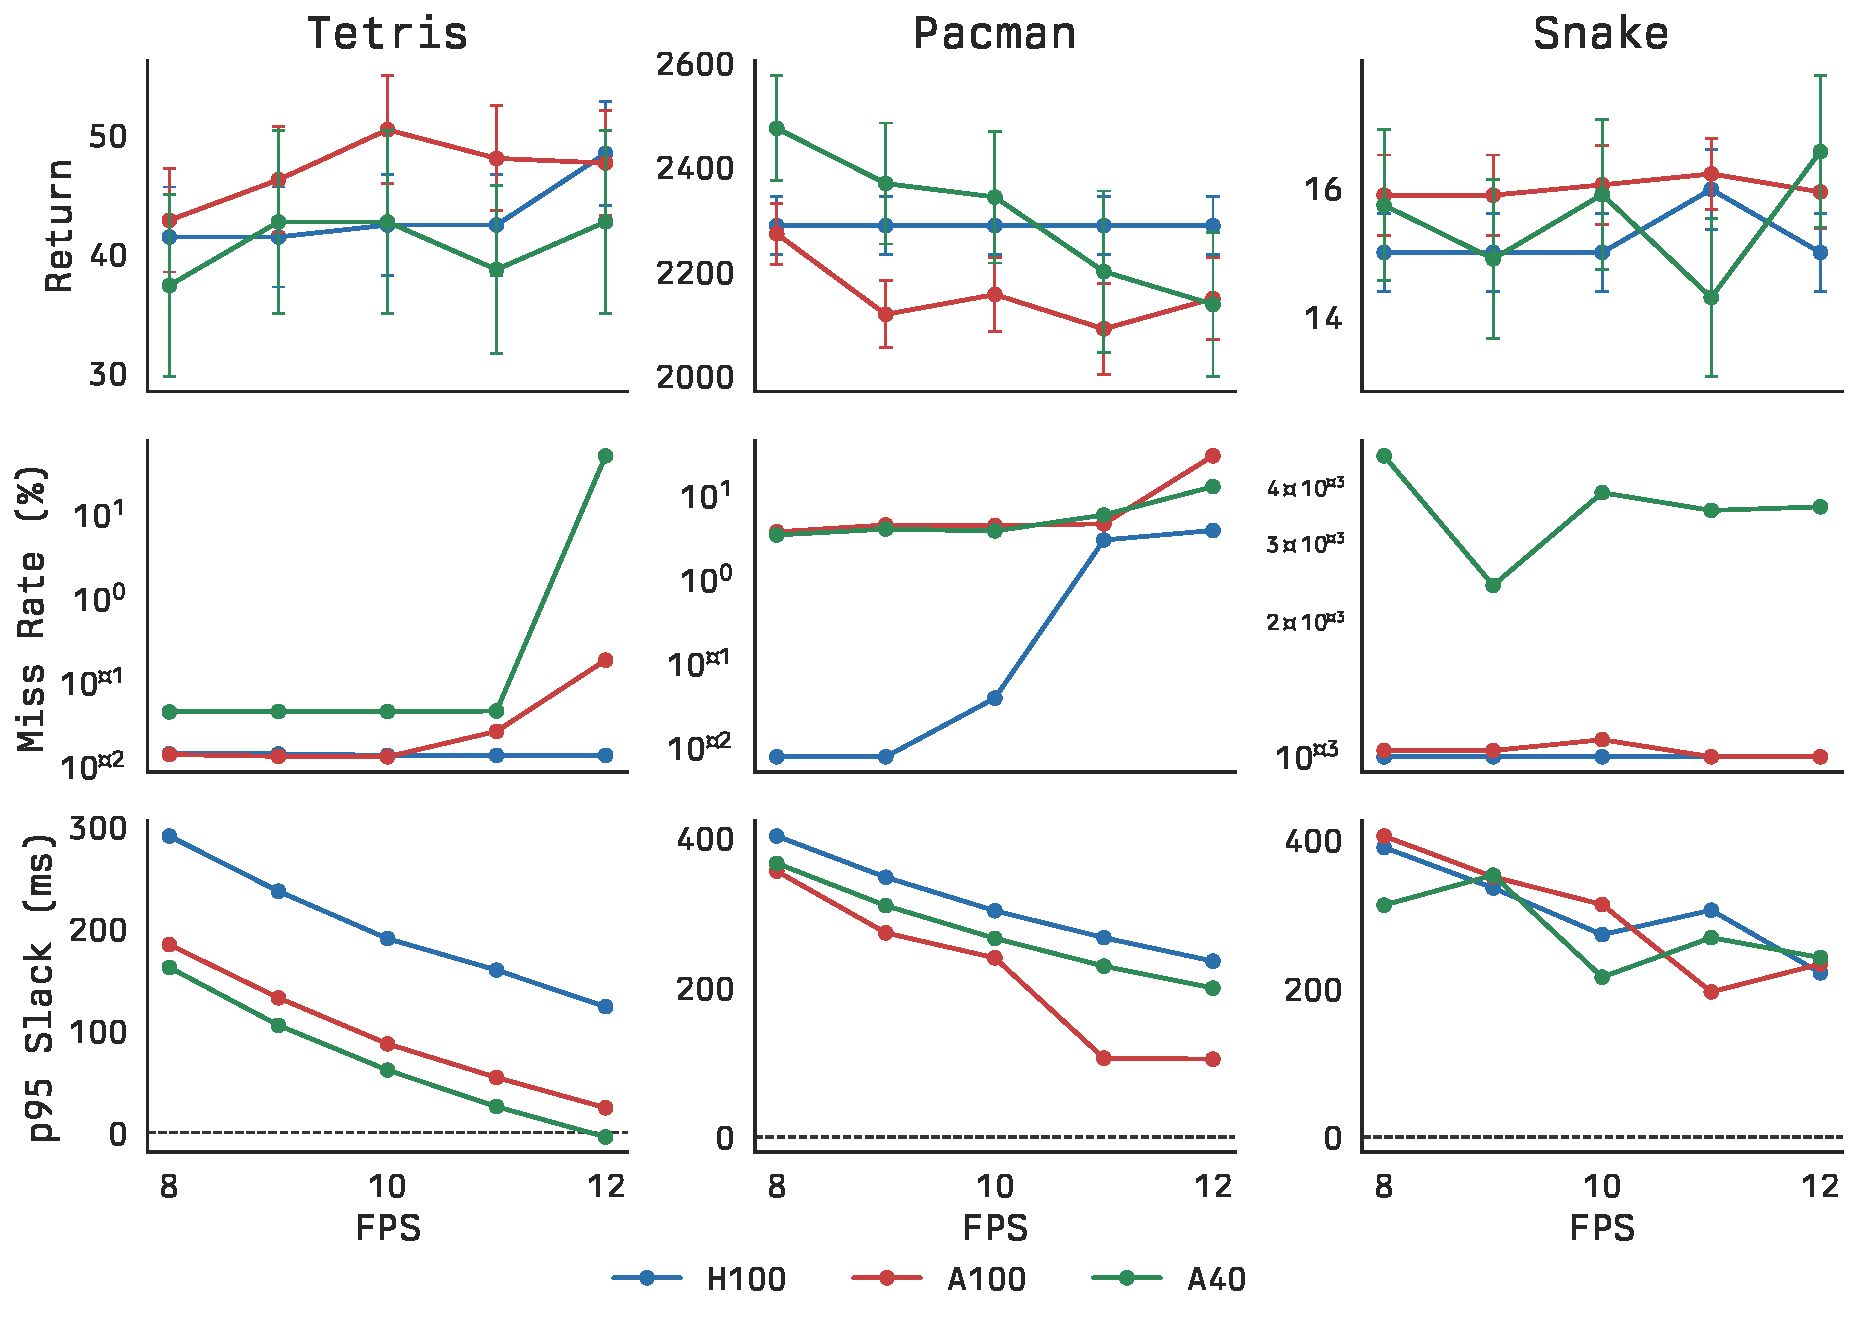
\includegraphics[width=\linewidth]{figures/deployment_appendix.pdf}
  \caption{Detailed two-GPU deployment breakdown across Tetris, Pac-Man, and Snake.
    \emph{Top row:} return vs.\ FPS with SE bars.
    \emph{Middle row:} deadline miss rate vs.\ FPS on a log scale.
    \emph{Bottom row:} p95 slack to the $K{=}4$ deadline.
    Each column is one environment; colors indicate hardware class.
    The qualitative transition is clear: Snake stays robust throughout, Tetris fails
    only near the tightest A40 regime, and Pac-Man is the most latency-sensitive
    environment overall.}
  \label{fig:deployment_appendix}
\end{figure}


\section{Additional Results and Ablations}
\label{app:ablations}

\todo{Suggested ablations:
(1) Gating with only raw game grid, no planner trunk features or value;
(2) Gating with only planner features, no spatial branch;
(3) Reward mode: raw vs.\ $\gamma^K$-discounted vs.\ per-step normalized;
(4) Sensitivity to entropy coefficient.}

%%%%%%%%%%%%%%%%%%%%%%%%%%%%%%%%%%%%%%%%%%%%%%%%%%%%%%%%%%%%

\section{Real-Time RL, SMDPs, and Committed-Action Training}
\label{app:rtrl_smdp}

\subsection*{The RTRL framework and its single-step restriction}

\citet{ramstedt2019rtrl} formalise real-time interaction via the
\emph{Real-Time Markov Decision Process} (RTMDP), which augments the environment
state with the action currently in execution:
$\mathbf{x}_t = (s_t, a_t)$,
where $a_t$ was selected one step earlier based on $s_{t-1}$.
The transition is
$p(\mathbf{x}_{t+1} \mid \mathbf{x}_t, \hat{a}_t) =
 p(s_{t+1} \mid s_t, a_t)\,\delta(a_{t+1} - \hat{a}_t)$,
passing the newly selected action $\hat{a}_t$ forward as the next state component.
This is equivalent to a \emph{constant 1-step delay MDP}~\citep{walsh2009delayed}:
the action the agent emits is applied one timestep later, and the policy must
learn to predict where the state will be when the action lands.

The framework is well-suited for lightweight policies whose evaluation time
fits within one frame.
For MCTS planning, however, the computation budget spans $K \in \{1,2,3,4\}$
frames ($111$--$444$\,ms at 9\,FPS).
A direct extension to a $K$-step delay MDP would require augmenting the state
with the $K$ most recent actions,
$\mathbf{x}_t = (s_t, a_{t-K+1}, \ldots, a_t)$,
whose size grows with planning depth.
Worse, under \emph{variable} $K$ the augmented state space would change
dimensionality at each meta-step, and the policy would need to predict the
state $K$ steps ahead through a chain of arbitrary committed actions---a
hard credit-assignment problem that does not arise in the 1-step case.

\subsection*{Training is a discrete SMDP; deployment is a genuine SMDP}

\paragraph{Simulation.}
In training the environment is synchronous: MCTS runs in zero simulated time.
Each meta-step proceeds by (1) gating chooses $K$, (2) $K{-}1$ committed
argmax steps execute, (3) the MCTS result is applied.
From the meta-policy's perspective this is a
\emph{Semi-Markov Decision Process}~\citep{puterman1994mdp} with \emph{deterministic}
holding time $\tau = K$ (chosen by the meta-action).
Successive meta-decisions are spaced $K$ environment steps apart and the
appropriate discount is $\gamma^K$, which is exactly the discount applied
in training.
Formally this is a discrete SMDP with options~\citep{sutton1999between}:
each $(K, \pi_{\mathrm{reflex}})$ pair defines an option of length $K$ terminating
with the MCTS action.

\paragraph{Deployment.}
In real-time deployment the holding time between meta-decisions is genuinely
stochastic: it equals $K \times T_{\mathrm{frame}}$ plus the actual MCTS
execution time, which varies with search dynamics.
This is a true SMDP in the continuous-time sense~\citep{puterman1994mdp}.
Our measurements show that the execution-time component is tightly concentrated
(H100: mean $122$\,ms, p95 $205$\,ms; A40: mean $197$\,ms, p95 $338$\,ms),
so the gap between the deterministic simulation discount $\gamma^K$ and the
true continuous-time discount is small, which is precisely why sim-to-real
transfer succeeds without retraining.

\subsection*{How committed-action training avoids state augmentation}

The central reason the $K$-step RTMDP state augmentation is unnecessary in
our framework is that \emph{the committed action at each intermediate step is
computed from the current state, not from a state $K$ steps ago}.
Specifically, the committed action at frame $t$ is
$a_t = \arg\max_a \pi_\theta(a \mid s_t)$, evaluated fresh in $\sim$2\,ms---well
within the $111$\,ms frame budget.
Only the MCTS result is stale: it was computed on $s_0$ (start of meta-step)
but applied at $s_K$ (after $K{-}1$ committed steps).
This staleness is explicitly modeled in training: the $K{-}1$ committed steps
actually execute in the environment before the MCTS action lands, so the policy
learns to handle the $K$-step gap without any state augmentation.

In the RTRL vocabulary, the committed-action component operates in the
\emph{turn-based} regime (computation time $\ll$ frame time, so the environment
effectively pauses during action selection), while the MCTS component operates
in a $K$-step delay regime whose effects are absorbed by the training curriculum
rather than by augmenting the state space.
The key property that makes this possible---and that the standard RTMDP does not
exploit---is that the intermediate policy $\pi_{\mathrm{reflex}}$ is a
\emph{deterministic function of the current state}, so its actions do not need
to be carried in the state to recover the Markov property.

%%%%%%%%%%%%%%%%%%%%%%%%%%%%%%%%%%%%%%%%%%%%%%%%%%%%%%%%%%%%

\newpage
\input{checklist.tex}

\end{document}
